\section{Methodology}
This section describes quorum systems based on the WoT graph, which
are the main building blocks for our BFT protocols. Protocols are
always between a client and a quorum. Every message must be signed by
a set of special nodes called {\em Quorum Cliques}, and stored in
another quorum called {\em KV quorum}. To write a key-value pair the
client performs the three step process:
\ifdefined\ABSTRACT
\footnote{Detailed protocols are described in the full paper.}
\fi
\begin{enumerate}
\item Collect timestamps from a quorum and choose the latest one,
\item Request to sign the message to a quorum in the {\em Quorum Cliques},
\item Write the signed message to a {\em KV quorum}.
\end{enumerate}
To read a key-value pair, the client performs the following process:
\begin{enumerate}
\item Collect key-value pairs from a {\em KV quorum}
\item Choose the latest one
\end{enumerate}
\ifdefined\ABSTRACT
\else
See the section \ref{Protocols} below for details.
\fi

In order to complete the system, authentication and signature schemes
based on a threshold cryptosystem are introduced in this section as
well.

\subsection{Quorum Cliques}
We follow the faulty clients (or dishonest writers) scenario described
in ``Byzantine Quorum Systems'' \cite{Delhi:1,Delhi:2}, which uses
signed messages with $b$-masking quorum systems to avoid equivocation.
\footnote{Aka double-spending in the blockchain world.}
In our system, such quorum system is constructed from maximal cliques
in the WoT graph.

If the graph $G$ contains some cliques and the starting node $s$ has
outdegree edges to the cliques within the $L$ distrance, i.e.,
\[
\exists (s, u) \in G.E, s.t., u \in QC \text{ and } dist(s, u) \le L \\
\]
where $QC$ is quorum cliques obtained by the algorithm {\sf GetQC}
\ref{GetQC},
it will construct a quorum to sign messages. Note that the quorum
depends on only the graph $G$. There are no other configuration data
or anything.
Such graph is constructed from the quorum certificates. 

\subsubsection*{Quorum Certificates}
Quorum certificates represent the proof of trustworthy. Each node
keeps its own quorum certificate along with the private key. 
A quorum certifiate consists of:
\begin{itemize}
\item a unique ID
\item a public key
\item a self signed signature over the ID and public key
\item a set of signatures signed by Quorum Cliques
\end{itemize}
When a node ($n_1$) is signed by another node ($n_2$) an edge is added
to the WoT graph, i.e., $G.E = G.E \cup \{(n_2, n_1)\}$.

The quorum certificate not only constructs the graph but also gives
permissions to clients to mutate the value.
Every {\sf write} request includes the client's quorum certificate
along with the self signed signature over the variable, timestamp and
value which we denote $\langle x, t, v \rangle$.
Each member of $QC$ verifies the signature and the quorum
certificate before it sends back the signed message. See algorithms
{\sf VerifyCollectiveSignatures} \ref{VerifyCollectiveSignatures} and
{\sf CheckQuorumCert} \ref{CheckQuorumCert}.

\subsubsection*{Sybil Attack}
When a node is compromised the node can try to make its own cliques
with made-up colluding nodes to outnumber the honest nodes. By the
algorithm {\sf GetQC} \ref{GetQC} which is used to verify the quorum
certificates and the collective signatures, a node cannot be a
member of more than one cliques, which means the compromised node has
to sever the trust links to other nodes itself to make links with the
colluding nodes, otherwise the clique can no longer be a member of a
quorum. If such a faulty clique disagrees with other cliques a
consensus will be no longer established until clients exclude the
compromised nodes.

\subsection{Key-value Store}
Once data is signed by quorum cliques it can be sent to other nodes
that are not necessarily members of the cliques. Such nodes can form
another quorum system and we call it {\em KV quorum}. The main purpose
of this quorum system is to make sure that clients can retrieve the
latest key-value. We no longer need the $b$-masking quorum as all
messages are signed by quorum cliques which have already handled the
faulty client case. {\em KV quorum} handles only $f$ benign faulty
nodes. The {\sf read} process writes back the latest message to nodes
that keeps old values:
\begin{enumerate}
\item The client collects $f + 1$ responses and chooses one which
  has the latest timestamp.
\item If some servers return an old value or {\em
    nil} the client will write back the latest value to those servers.
\end{enumerate}
\ifdefined\ABSTRACT
\else
See ~\ref{rw} for the actual protocols.
\fi
For load balancing, {\em KV quorum} is typically chosen from $U
\setminus\; QC$.

Each member of {\em KV quorum} must check equivocation and the
permission of mutation (TOFU), when it receives the signed
transaction.

\subsubsection*{Equivocation Check / Revocation}
Revocation is the only way to keep the system sound in the long
run. Keeping the number of faulty nodes within the quorum threshold is
the key to the soundness of the system.

Each node severs the trust link independently without consulting
others when it detects a node that has signed both $\langle x,t,v
\rangle$ and $\langle x,t,v' \rangle$ s.t.  $v \neq v'$. Also servers
revoke clients when it detects a client signing different values with
the same timestamp as well. Once a node is revoked, it will be
excluded from the WoT graph forever and there is no way to restore it.
See algorithm {\sf CheckEquivocation} \ref {CheckEquivocation} for
the equivocation check.

\subsubsection*{TOFU Policy}
The system enforces the TOFU policy on every write request. If the
slot is empty each node in the KV quorum will simply store the
data. If the slot already has data, the node first retrieves the
latest data and check if the signer is the same as the one of the
requested data.  See {\sf CheckTOFU} \ref{CheckTOFU} for the
algorithm to check the TOFU policy.

\subsection{Threshold Password Authentication ($\mathcal{TPA}$)}
\label{auth}
The quorum system based on the WoT graph guarantees data
integrity. The TOFU policy with the quorum certificate prevents
unauthorized mutations. The collective signatures make it possible to
check equivocation. All those functions rely on the digital signature
scheme therefore managing the signing key is significantly
important for this system. We use a threshold password authentication
($\mathcal{TPA}$) for:
\begin{itemize}
\item enrolling nodes to the system
\item recovering from a key-loss situation
\item sharing an ID with multiple devices
\item data secrecy (roaming encryption)
\end{itemize}
$\mathcal{TPA}$ is immune from offline dictionary attacks (as long as
the number of compromised servers is less than the threshold). The
authentication protocol is similar to \cite{ford} by Ford and Kaliski,
but the shared secret is calculated by Shamir's Secret Sharing (SSS)
\cite{shamir}.\\

To set up the {\em shares} the client generates a random polynomial
for $(t, n)$ SSS over a prime field $\mathbb{Z}_q$, s.t.,
\[
  f(x) = \sum_{i=0}^{t-1}a_ix^i \bmod q
\]
then calculates $n=|Q|$ pairs $(i,f(i)), i = 1..n$. The shared secret
is $S = f(0)$. Each {\em share} will be $\langle i, y_i, v_i, t_i
\rangle$,
where:
\begin{align*}
  y_i &= f(i) \\
  v_i &= g_{\pi}^{Ss_i} \bmod p \\
  s_i &= \text{OS2I}(h(password, t_i)) \\
  g_{\pi} &= \pi^2 \bmod p \\
  \pi &= \text{OS2I}(h(password))
\end{align*}
$p$ and $q$ are prime numbers such that $p = 2q + 1$ (i.e., $p$ is a
safe prime). $t_i$ is a salt. The random polynomial must be generated
randomly for each password.\\

To get a password authenticated:
\begin{enumerate}
\item The client generates a random number
  $a \xleftarrow{\mathcal{R}} \mathbb{Z}_q$
  and calculates $X$ from the password:
  \[
    X = g_{\pi}^a \bmod p
  \]
  then broadcast it to a quorum $Q$.

\item Each quorum member returns:
  \[
    Y_i = X^{y_i} \bmod p
  \]
  with the salt $t_i$.

\item The client collects $t$ responses from the quorum ($\mathcal{T}
  \subseteq Q$), and
  calculates:
  \[
    G_S = \prod_{j \in \mathcal{T}}Y_i^{\lambda_j} \bmod p
  \]
  where each $\lambda_j$ is the lagrange interporate:
  \[
    \lambda_j = \prod_{l \in \mathcal{T} \setminus \{j\}}
    i_l / (i_l - i_j) \bmod q.
  \]
  Then, generate another random number $a' \xleftarrow{\mathcal{R}}
  \mathbb{Z}_q$ and for each server $i \in \mathcal{T}$, calculate and
  send back:
  \[
    X_i = G_S^{s_ia'} \bmod p
  \]
  where
  \[
    s_i = h(password, t_i)
  \]

\item Each quorum member($\in \mathcal{T}$) generates a random exponent
  $b_i \xleftarrow{\mathcal{R}} \mathbb{Z}_q$
  for a DH session key:
  \[ K_i = X_i^{b_i} \bmod p \]
  and encrypts the proof ($P_i = Sig_i(\centerdot)$):
  \[
    Z_i = E_{h(K_i)}(P_i, X || Y_i)
  \]
  then sends it back to the client with
  \[
    B_i = v_i^{b_i} \bmod p.
  \]

\item The client decrypts $Z_i$ with
  \[
    K_i = B_i^{aa'} \bmod p
  \]
  and gets:
  \[
    (P_i, N) = D_{h(K_i)}(Z_i).
  \]
  Check if $N = X||Y_i$ to make sure both parties have shared the
  session key correctly. 
\end{enumerate}
We use $\{P_i\}_{\{i \in \mathcal{T}\}}$ as the proof of
authentication which will be attached to protocol messages and checked
at each node during the {\sf read / write / register} protocols. The
signed data in each $P_i = Sig_i(\centerdot)$ depends on those
protocols.

\ifdefined\ABSTRACT
Here is a brief explanation of correctness
\footnote{See the full paper for a security analysis.}.
Assume $\{Y_i\}_{\{i \in \mathcal{T}\}}$ is correctly calculated,
$G_S$ will be:
\[
  G_S = \prod_{j \in \mathcal{T}}Y_i^{\lambda_j} = g_{\pi}^{a \sum_{j
      \in \mathcal{T}} f(j) \lambda_j} = (g_{\pi}^S)^a \bmod p
\]
and by raising $s_i = h(password, s_i)$ to $G_S$, we get:
\[
  X_i = G_S^{s_i} = (g_{\pi}^{Ss_i})^a \bmod p
\]
which must be the same as $v_i^a \bmod p$ for each $i \in
\mathcal{T}$ iff the correct password ($g_{\pi}$) is given at the
step 1. With each $B_i = v_i^{b_i} \bmod p$, the client and servers
share DH keys $K_i = g_{\pi}^{Ss_iab_i} \bmod p$.
\else
See Appendix \ref{tpa} for correctness and security analysis of
$\mathcal{TPA}$.
\fi

\subsubsection*{$\mathcal{TPA}$ for Enrollment}
$\mathcal{TPA}$ is used to enroll new nodes to the system so it can
recover from a key-loss situation and support multiple devices per
user.\\

\noindent
Enrollment:
\begin{enumerate}
\item Generate a unique ID and a key pair,
\item Send the certificate signing request to a quorum with the
  $\mathcal{TPA}$ {\em shares} to get a quorum certificate.
\end{enumerate}

\noindent
Key recovery / secondary key generation:
\begin{enumerate}
\item Generate a new key pair with the existing ID,
\item Do the password authentication and get a proof,
\item With the proof, send the new certificate to a quorum to get a new
  quorum certificate.
\end{enumerate}
\ifdefined\ABSTRACT
\else
See \ref{register} for the actual protocols.
\fi

\subsubsection*{$\mathcal{TPA}$ for Data Secrecy}
The system provides a roaming service to store and access encrypted
data. Users encrypt a value at a node then send the encrypted value
to a quorum. They can decrypt the value at any node with the
password. The password is stored along with $\langle x, t, v \rangle$.
The encryption key is $h(g_{\pi}^S)$. $S$ (and the random polynomial
as well) has to be randomly generated everytime the data is encrypted
at a client.

To decrypt the data the user specifies the variable $x$ along with the
password then the client starts the threshold password authentication
process first to get the proof. With the proof the client proceeds the
{\sf read} process and decrypts the value with the above key.

With this roaming scheme, BFTKV can be a secure vault that is not only
fault-tolerant for high availability but immune to single point of
failures. The same kv storage can be used to keep both public / private
keys without relying on a separated KMS.

\subsection{Distributed Signing}
Some crypto-currency platforms still use simple digital signature
schemes to sign transactions. If private keys are stolen all assets
can be transferred to someone's address without authorization from
the original users. One of ways to mitigate such situation is to
use {\em multi-sig}. With the multi-sig scheme multiple parties need
to be involved in the signning process. Most systems adopt multi-sig
as an add-on security measure to the blockchain technologies. BFTKV
natively supports distributed signing schemes based on threshold
cryptography, which is compatible with the standard algorithms
therefore the verifiers do not need to change the way to process the
transactions.

As a PKI platform, protecting CA's private keys must be the most
important {\em feature}. At the same time, certificate signing
requests should be processed quickly and automatically. The
distributed signing feature satisfies those conflicting requirements.

The system takes advantages of the distributed platform to make a
signature without revealing the private key. Once the key is
distributed among quorum members, the complete private key will never
appear at any server or client. The system supports three
signature algorithms: RSA (PKCS1.5), DSA and ECDSA. Our scheme takes
existing keys as-is and distributes it to multiple servers, which will
make it easy to migrate from existing systems.

\subsubsection*{RSA}
\label{thrsa}
It is straightforward to construct a $(n, n)$ ``threshold'' scheme with
RSA \cite{garay,rabin}. Decompose the private key $d$ into $\{d_i\}_{i =
1..n} \; \text{s.t., } d = \sum_{i=1}^{n} d_i \bmod \varphi(N)$, and the
signature is calculated from partial signatures $S_i = M^{d_i} \bmod
N$:
\[
  S = \prod_{i=1}^{n} S_i = M^d \bmod N.
\]

To convert the $(n, n)$ threshold scheme to a somewhat $(t, n)$
threshold scheme, we construct the partial keys recursively. In the
following tree, if a node (2) is a faulty its key will be compensated
by other nodes (1, 3, 4, 5) with the keys (21, 23, 24, 25)
respectively, i.e., $S = \prod_{i \in \{1,2,3,4,5\}} S_i \bmod N$
where $S_2 = \prod_{i \in \{21,23,24,25\}} S_i \bmod N$.

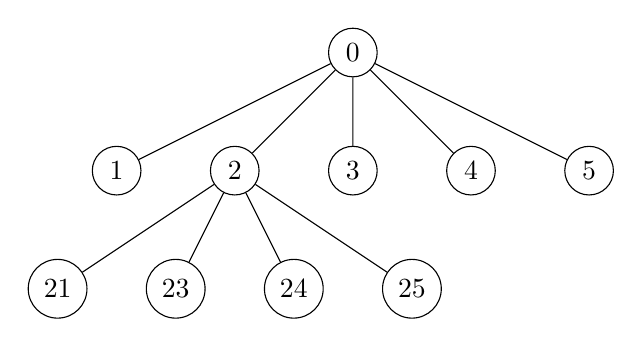
\begin{tikzpicture}[every node/.style={draw,circle}]
  \node (0) {0}
  child {node(1) {1}}
  child {node(2) {2}
    child {node(21) {21}}
    child {node(23) {23}}
    child {node(24) {24}}
    child {node(25) {25}}
  }
  child {node(3) {3}}
  child {node(4) {4}}
  child {node(5) {5}};
\end{tikzpicture}

The number of keys stored in each node will be increased exponentially
as $n - k$ becomes big. Up to $(7,10)$ threshold seems practical.

\subsubsection*{DSA, ECDSA}
BFTKV implements a DSS threshold scheme introduced by Gennaro et
al.\ \cite{Gennaro}.
Since the scheme has a restriction such as $n \geq 2t$ in the $(t,
n)$-threshold scheme, we no longer be able to use the quorum threshold
for $(t, n)$, but we follow the protocols between the client and a
quorum. The signing protocol consists of three phases:
\begin{enumerate}
\item Collect joint shared secrets generated by each quorum member:
  $\{(i, f_j(i)) | f_j(0) = k_j\}_{\{i = 1 \dots n, j \in Q\}}$
\item Distribute the secrets to the quorum and calculate
  $r=g^{k^{-1}} \bmod p \bmod q$ where $k$ is the
  joint Shamir's shared secret (i.e., $k = \sum k_i$)
\item Distribute r to the quorum and calculate $s=k(m+xr) \bmod q$
  from each $s_i=k_i(m+x_ir) \bmod q$ returned from each quorum member
\end{enumerate}
